\subsection{2J0T Control region}

The 2J0T control region is dominated by $W$+light flavor jets (and \QCD) events. In order to test the modelling of this background component, the distributions of several kinematic variables are studied. The distributions of the relevant background processes are normalized to their MC-predicted yields, summed up, and compared to the distributions from data.  Figure~\ref{fig:Jets2J0T} shows the p$_{T}$ and absolute value of $\eta$ distributions of the "light" jet (here: the more forward jet) and the "b-tagged" jet (here: the more central jet). Figure~\ref{fig:Mu_MET_2J0T} shows the distribution of the transverse momentum and the rapidity of the muon, the missing transverse energy of the event and the transverse mass of the neutrino-muon system.



\begin{figure}[hbpt]
\begin{center}
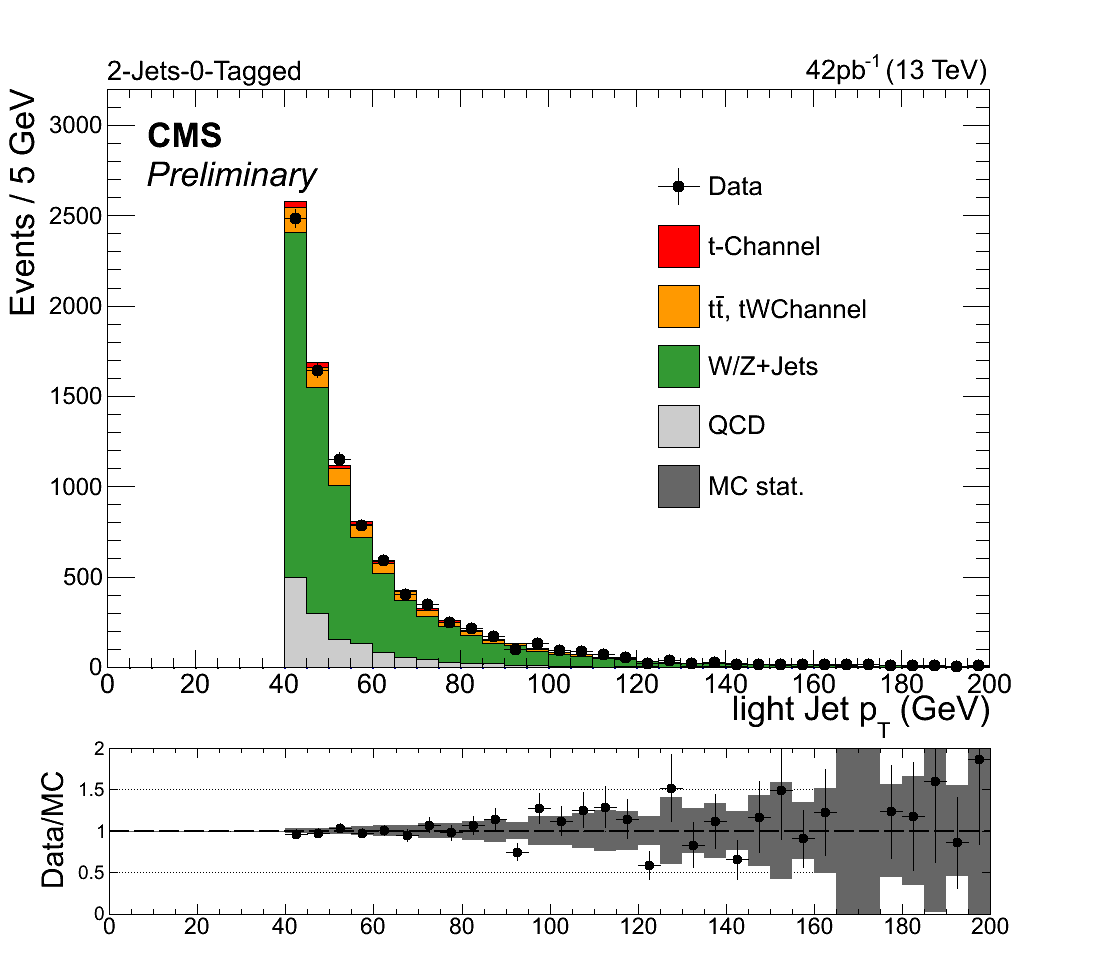
\includegraphics[width=0.45\textwidth,height=0.4\textwidth]{figures/2J0T/Sep8/lightJetPt.png}
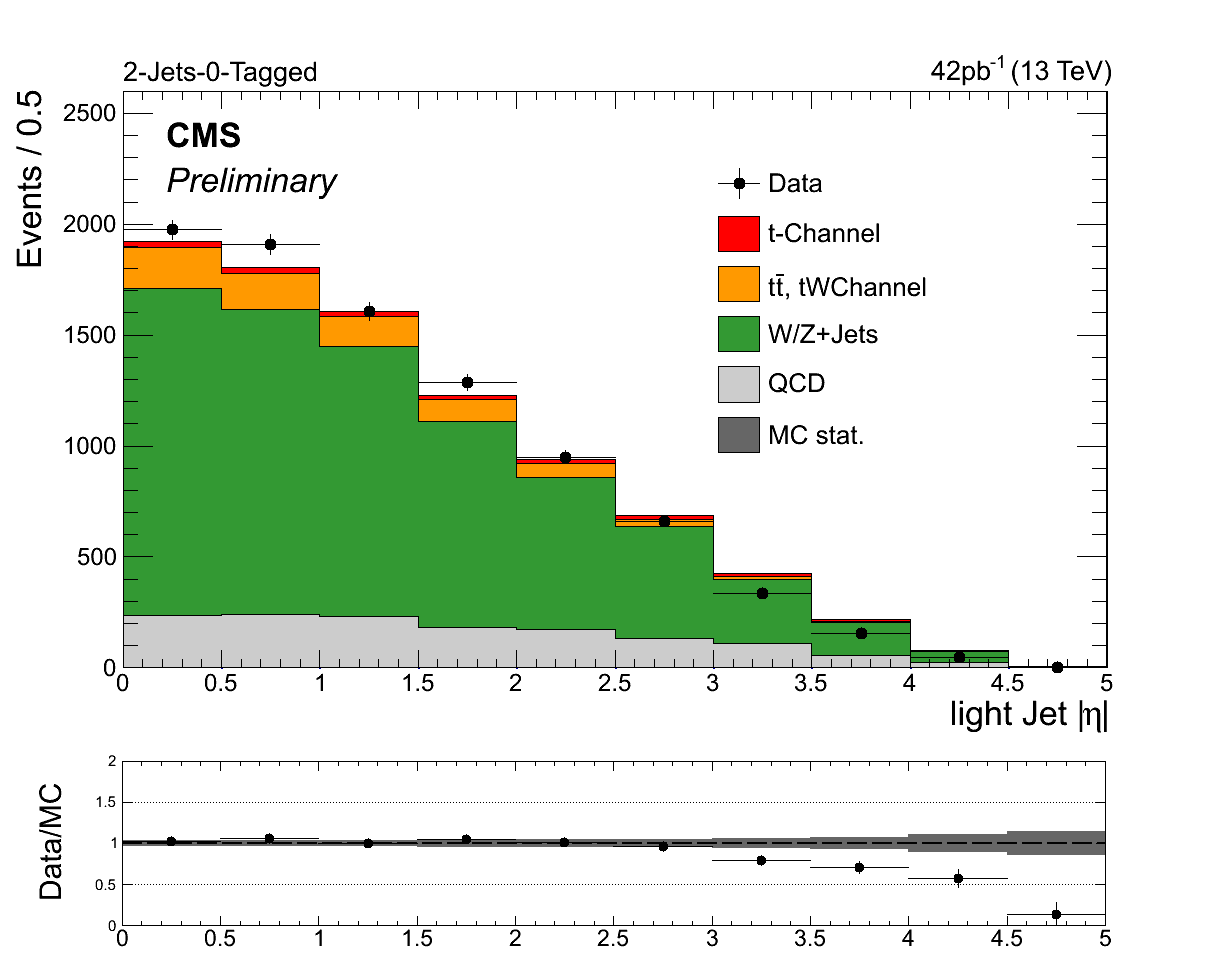
\includegraphics[width=0.45\textwidth,height=0.4\textwidth]{figures/2J0T/Sep8/lightJetEta.png}
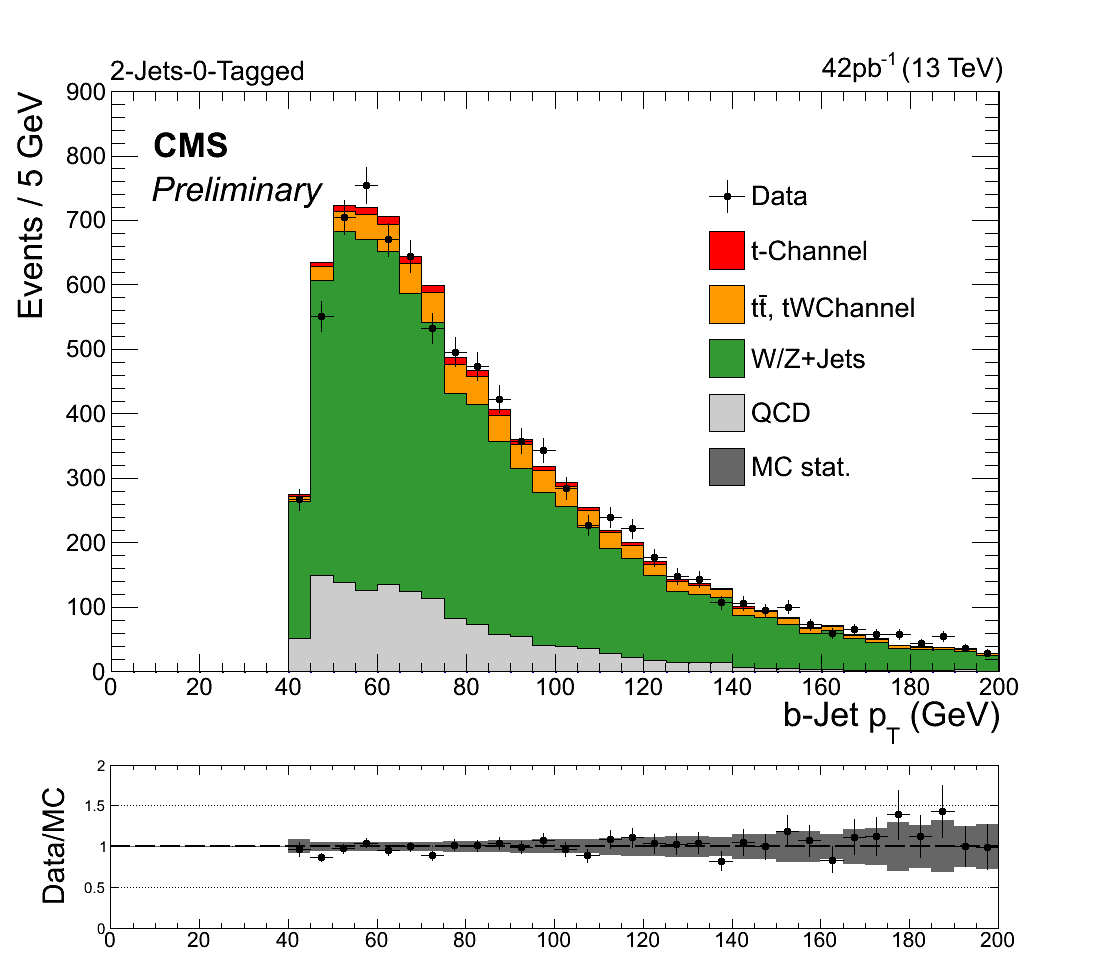
\includegraphics[width=0.45\textwidth,height=0.4\textwidth]{figures/2J0T/Sep8/bJetPt.png}
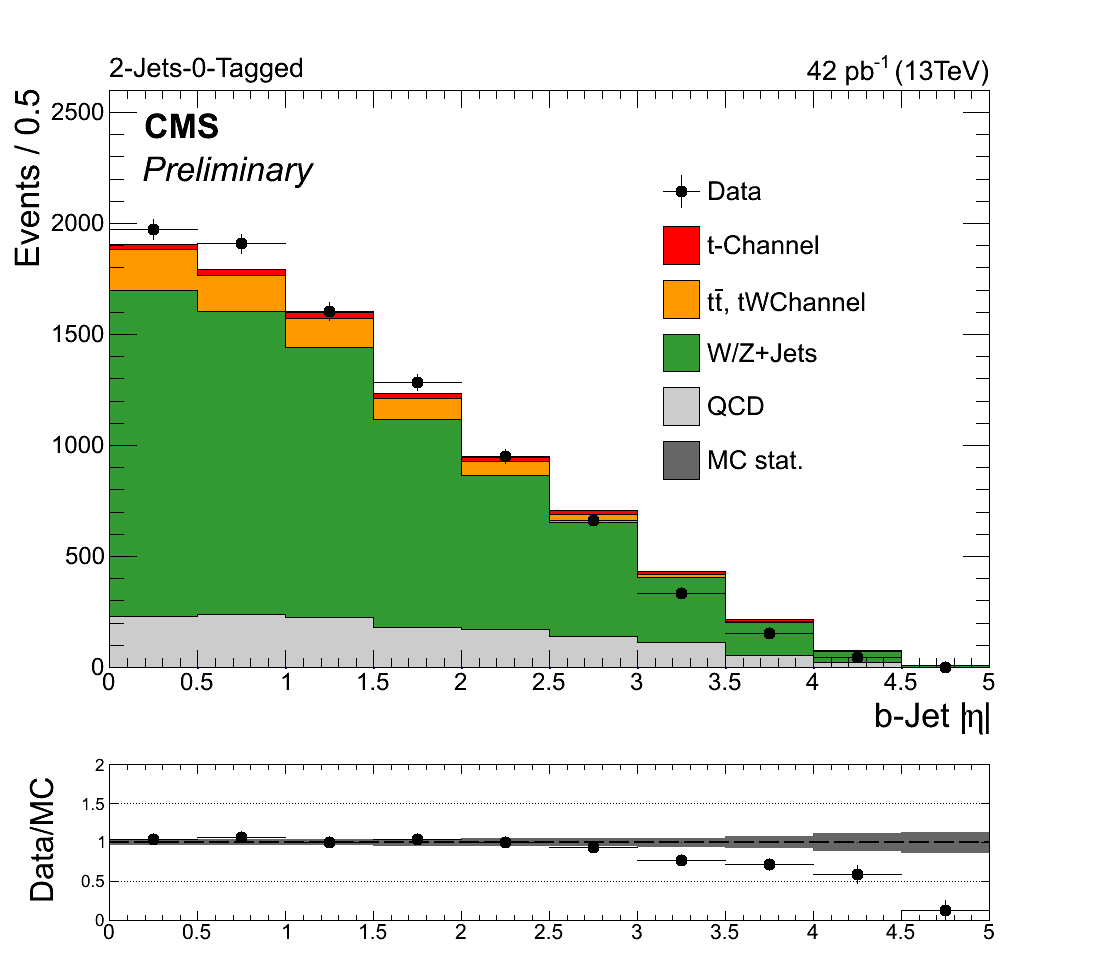
\includegraphics[width=0.45\textwidth,height=0.4\textwidth]{figures/2J0T/Sep8/bJetEta.png}\hfill
\caption{\label{fig:Jets2J0T}p$_{T}$ (left) and absolute value of $\eta$ (right) distributions of the "light" jet (upper row) and the "b" jet (lower row) in the 2J0T region. As this is the 0T region, the "b" jet refers to the jet with higher $p_{\mathrm{T}}$ and the "light" jet to the other jet.}
\end{center}
\end{figure}


\begin{figure}[hbpt]
\begin{center}
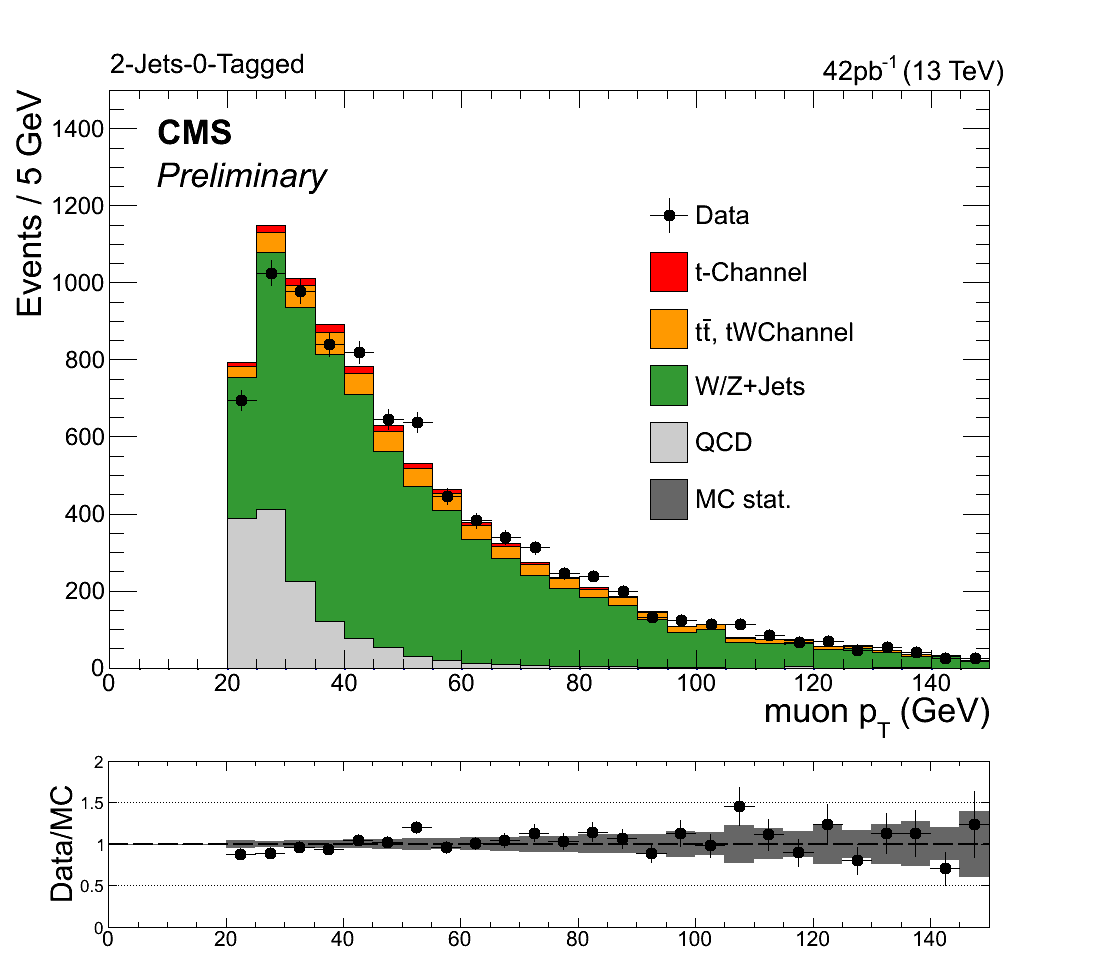
\includegraphics[width=0.45\textwidth,height=0.4\textwidth]{figures/2J0T/Sep8/muPt.png}
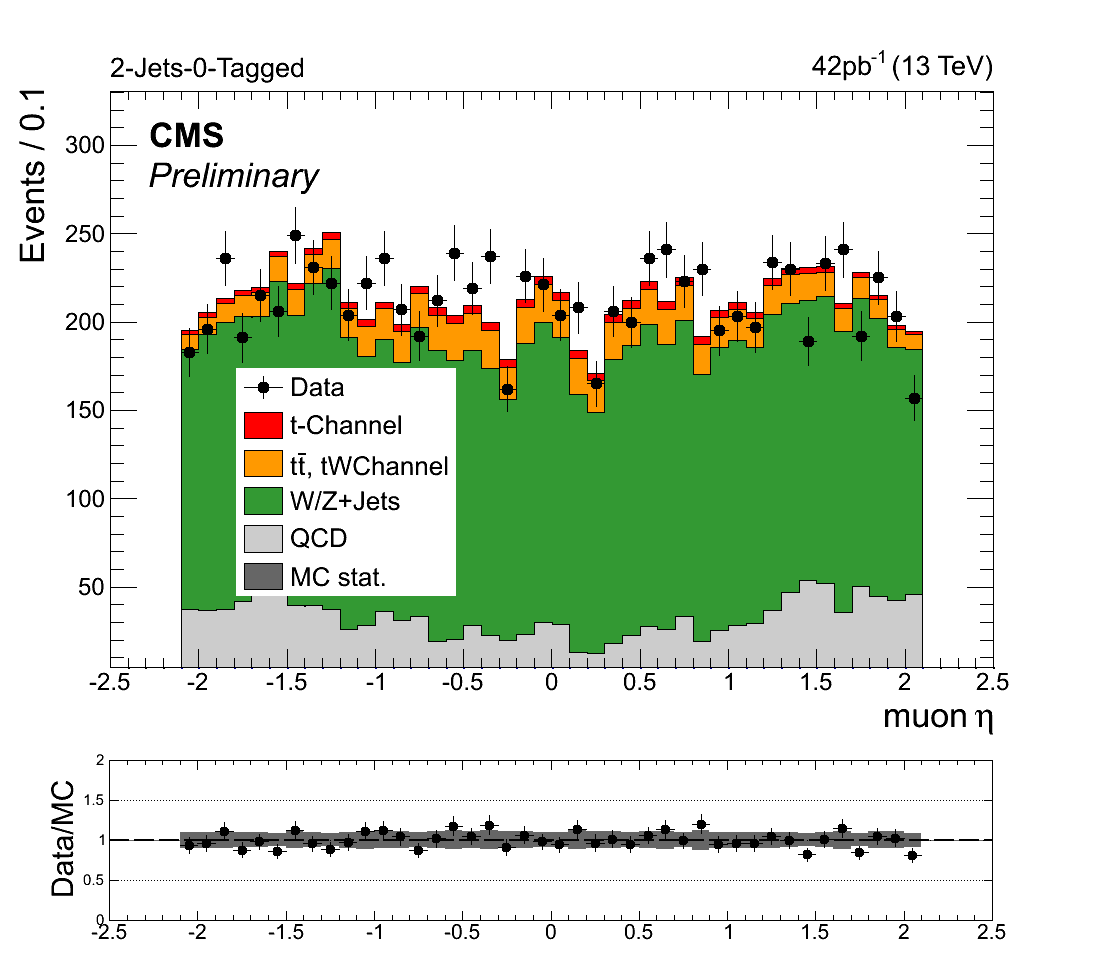
\includegraphics[width=0.45\textwidth,height=0.4\textwidth]{figures/2J0T/Sep8/muEta.png}
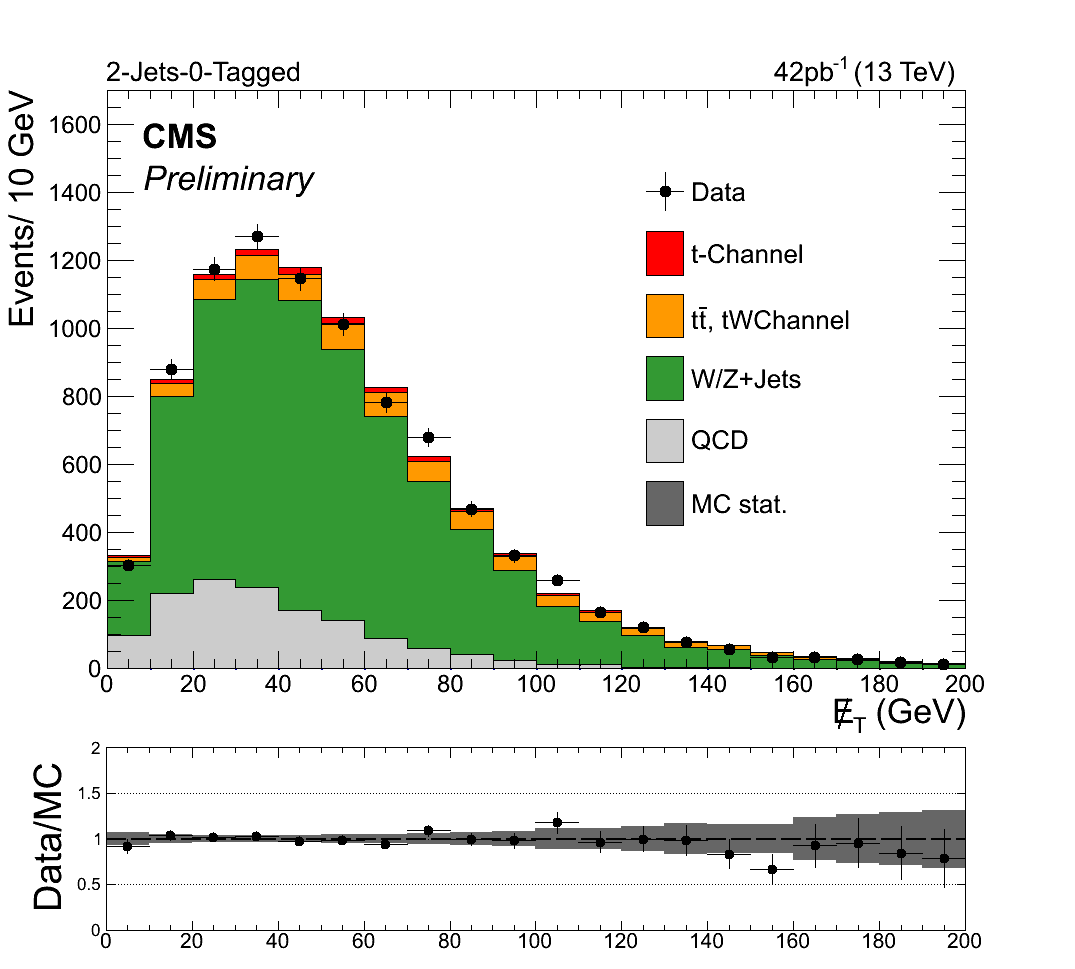
\includegraphics[width=0.45\textwidth,height=0.4\textwidth]{figures/2J0T/Sep8/metPt.png}
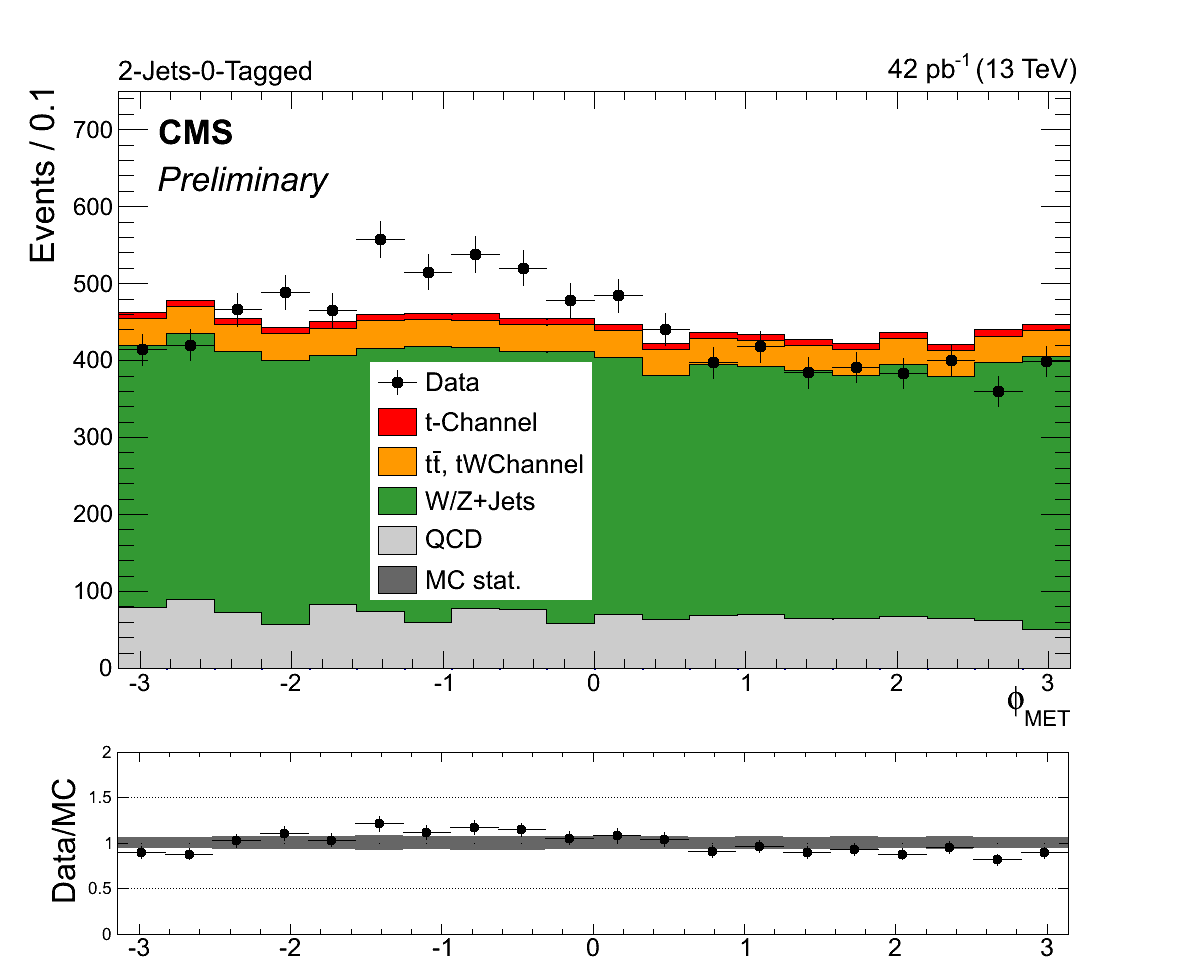
\includegraphics[width=0.45\textwidth,height=0.4\textwidth]{figures/2J0T/Sep8/metPhi.png}
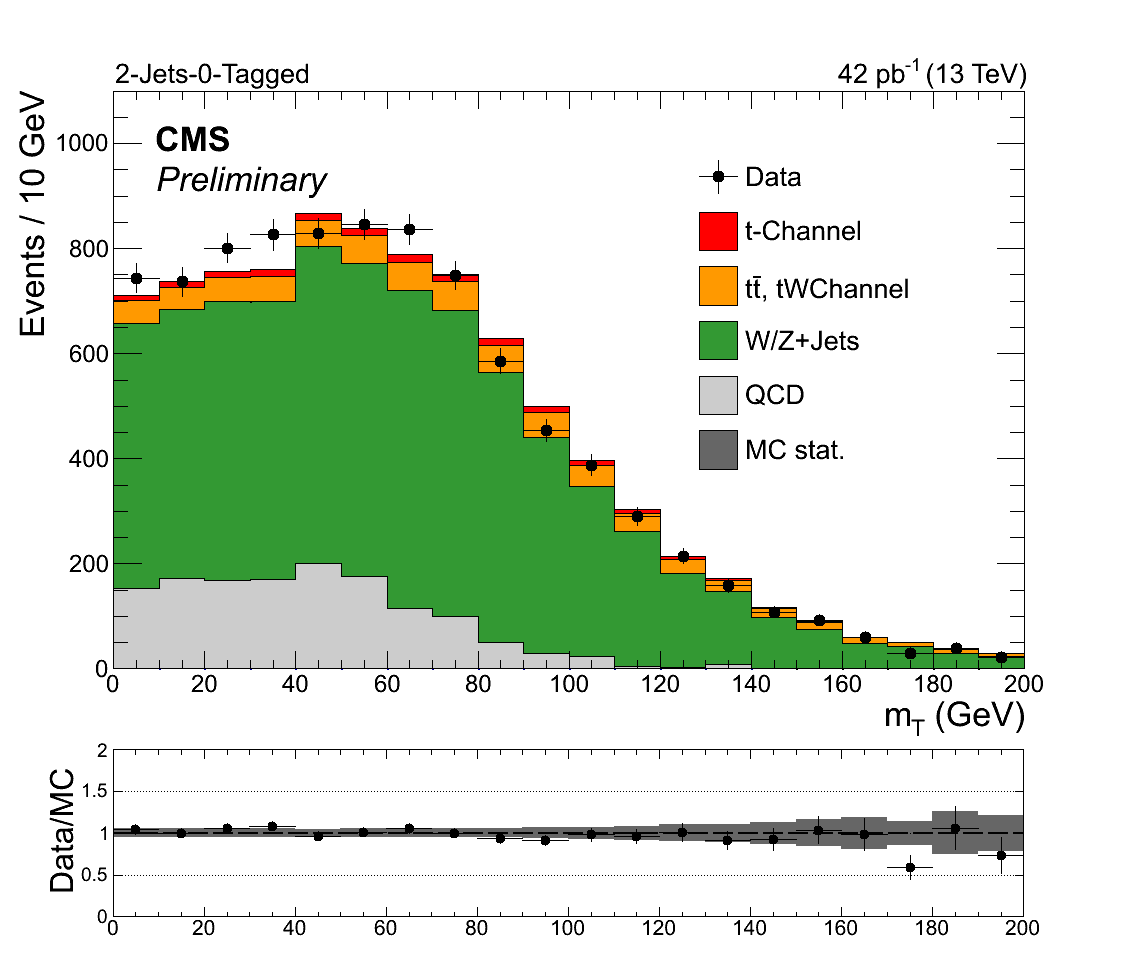
\includegraphics[width=0.45\textwidth,height=0.4\textwidth]{figures/2J0T/Sep8/mtW.png}\hfill
\caption{\label{fig:Mu_MET_2J0T} Distributions of muon p$_{T}$ (upper left) and $\eta$ (upper right) in the 2J0T region and \met (middle left) and \met-$\phi$ (middle right) and \mT (bottom) in the 2J0T region.}
\end{center}
\end{figure}





%\begin{figure}[hbpt]
%\begin{center}
%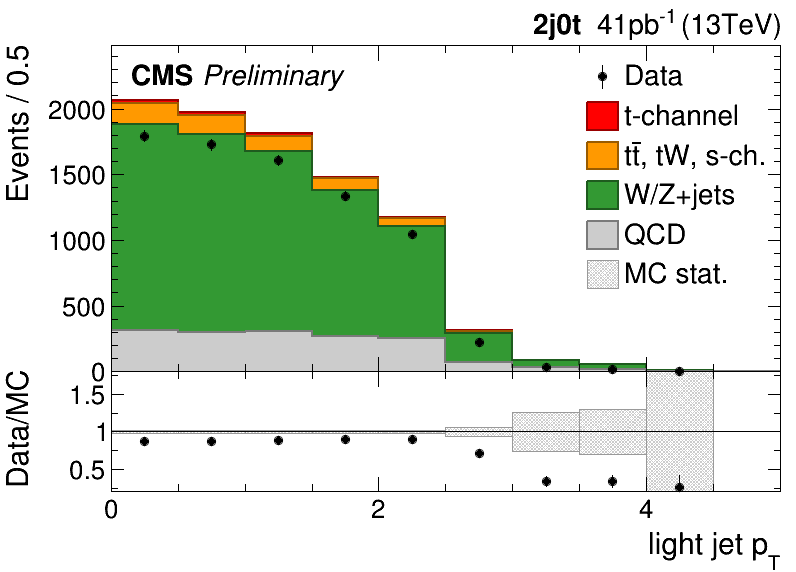
\includegraphics[width=0.45\textwidth]{figures/2J0T/2j0t_ljet_abseta_qcdnone.png}
%\caption{\label{fig:etajprime2J0T}$\eta_{j'}$ distribution in 2J0T}
%\end{center}
%\end{figure}

\clearpage

\subsection{3J2T Control region}

The 3J2T control region is dominated by \ttbar~ events. In order to test the \ttbar~simulation again the distributions of several kinematic variables from simulation are compared to the distributions from data. 


\begin{figure}[hbpt]
\begin{center}
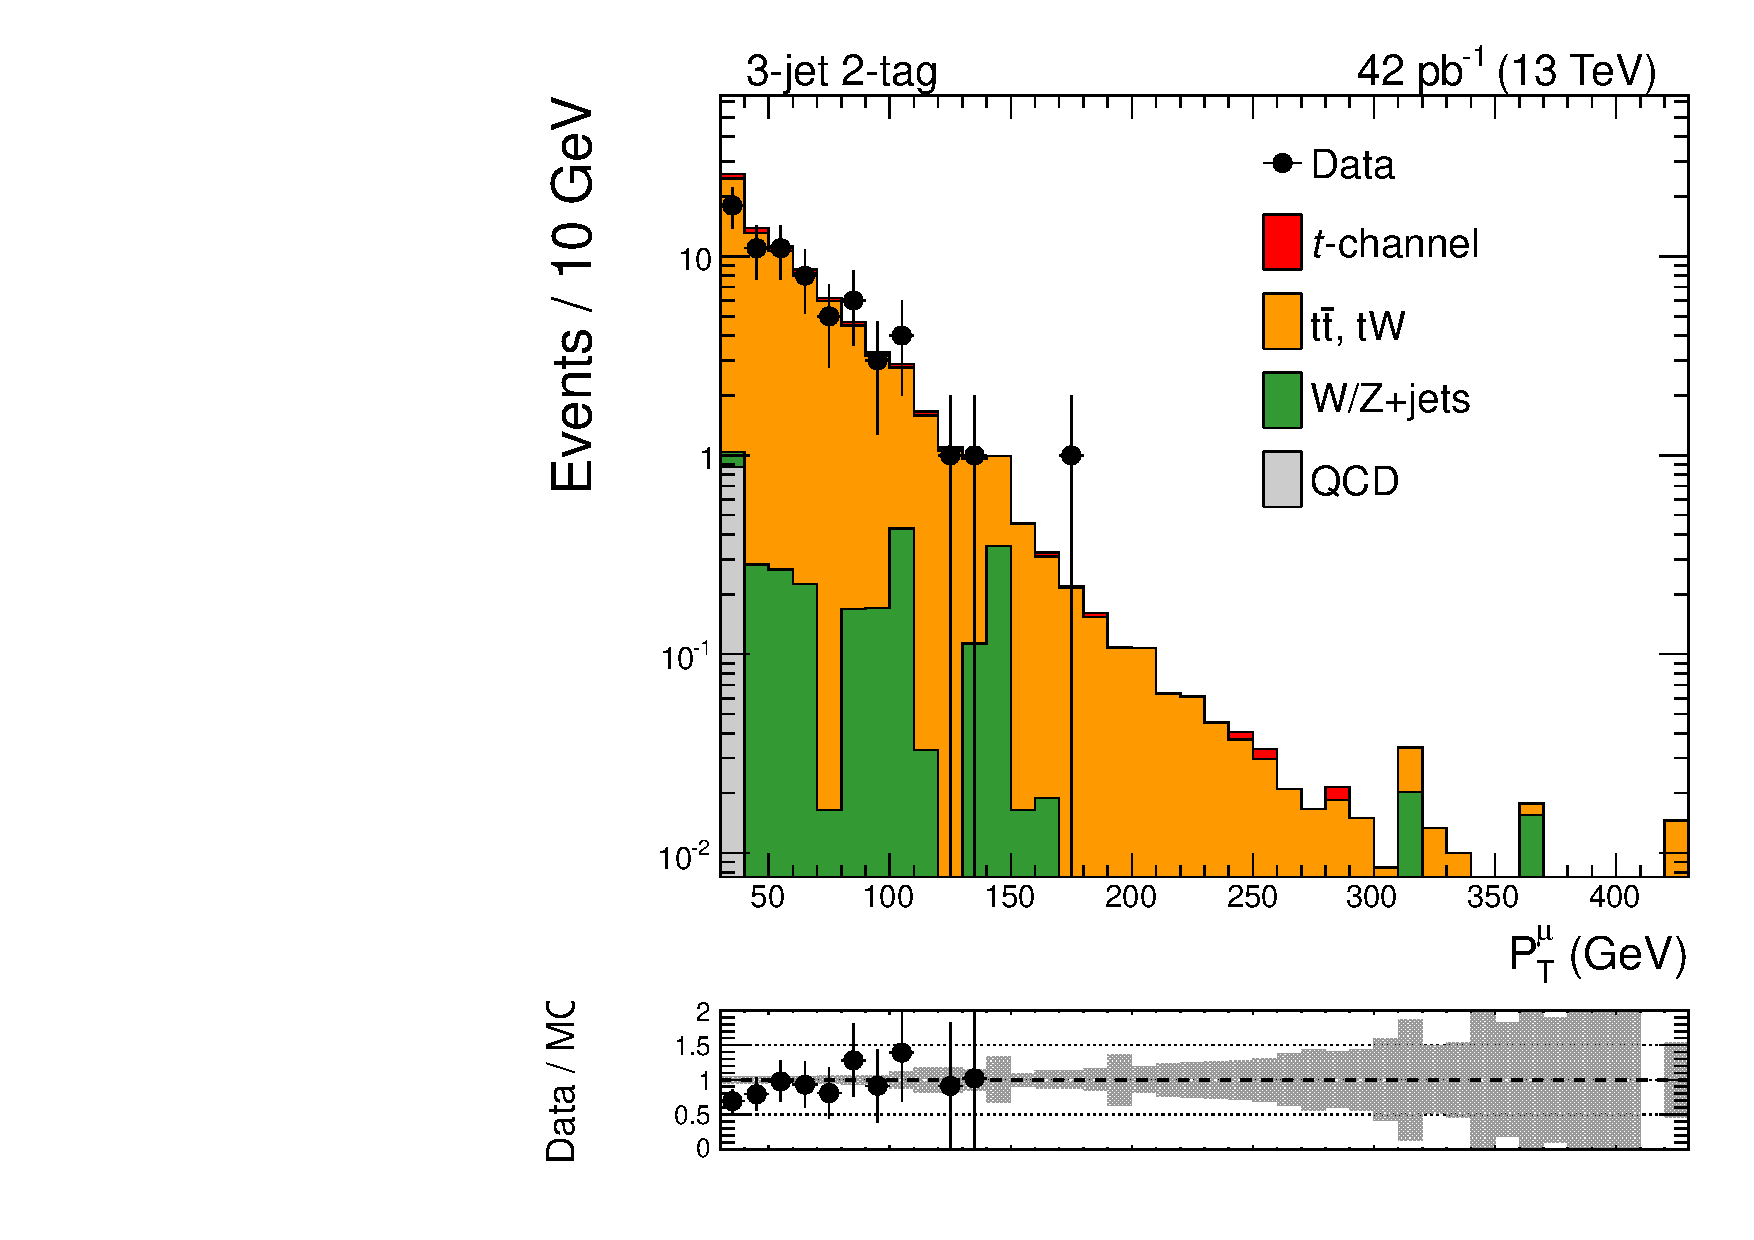
\includegraphics[width=6.5cm]{figures/3J2T/3j2t_muPt.pdf}
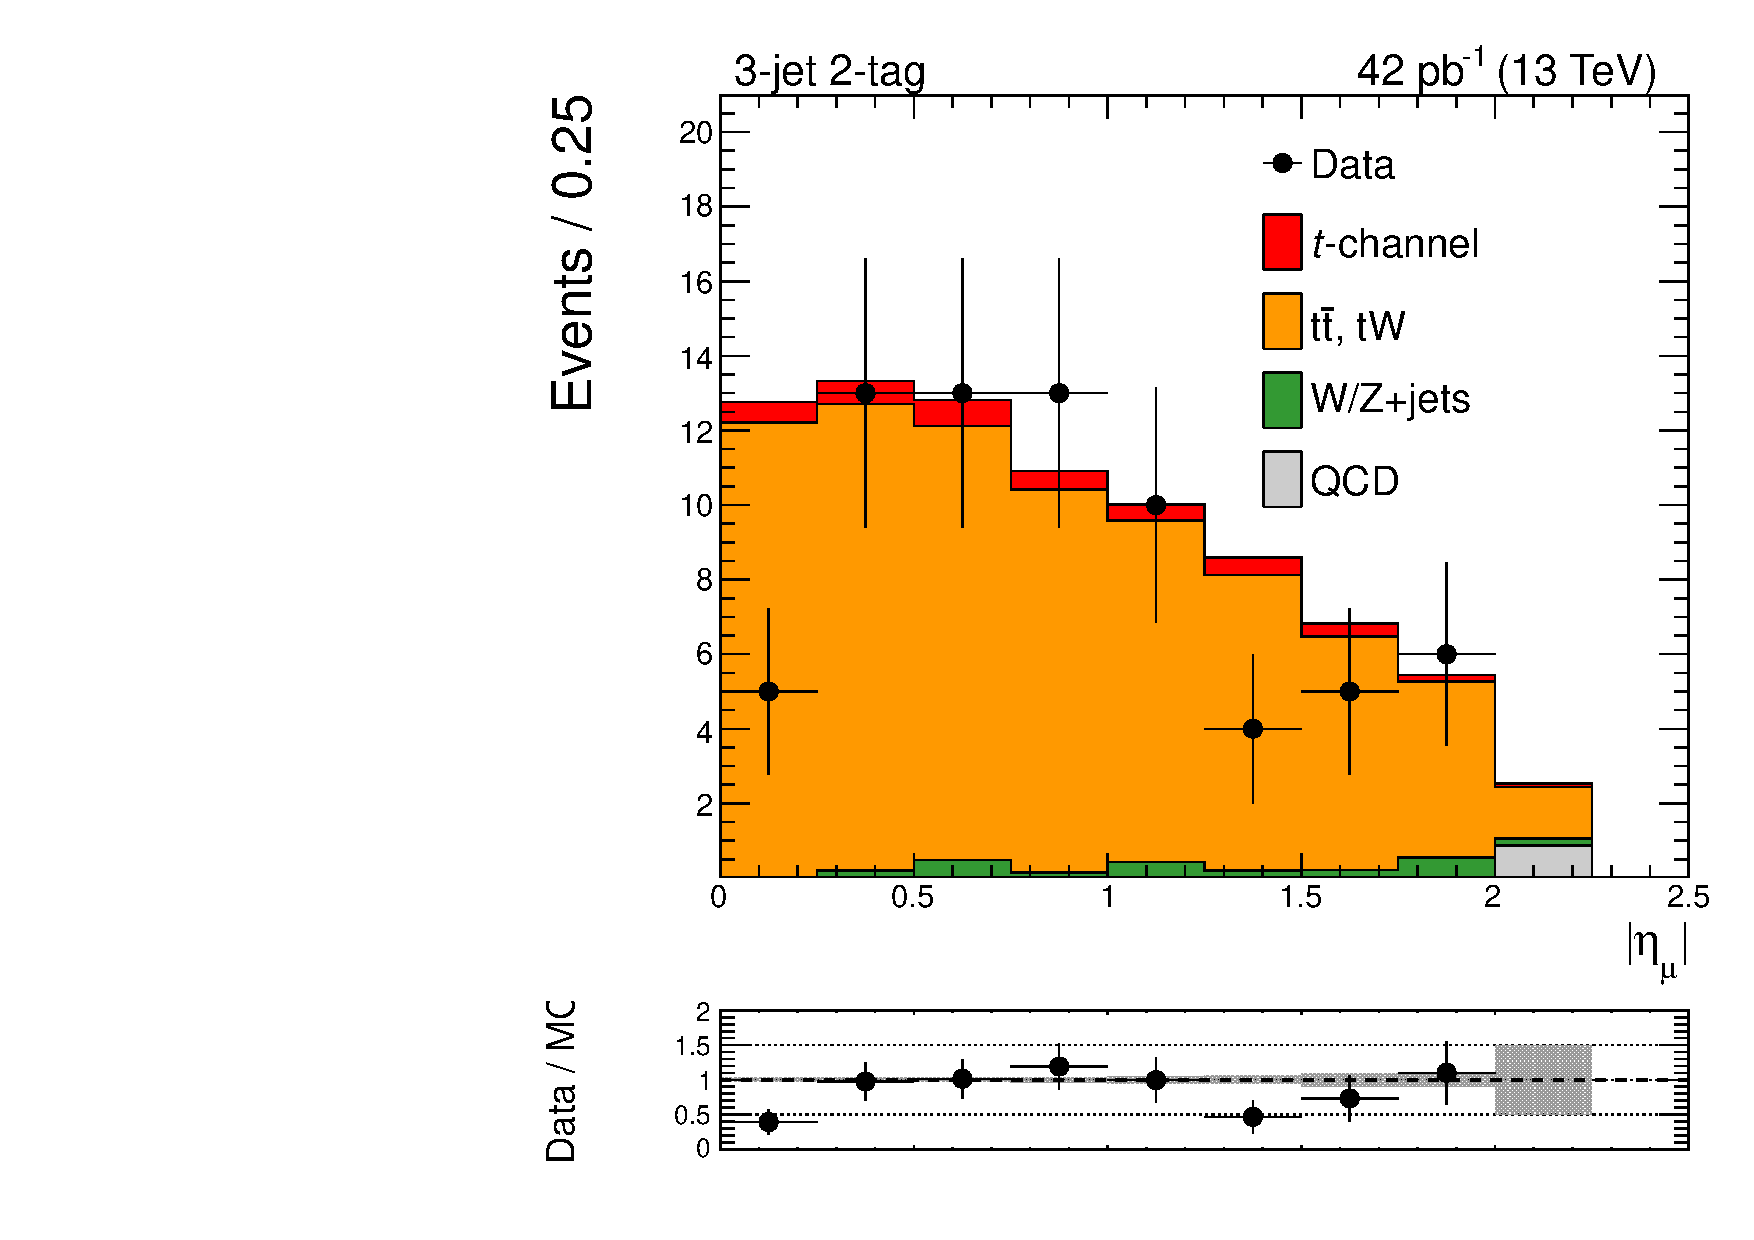
\includegraphics[width=6.5cm]{figures/3J2T/3j2t_mueta.pdf}
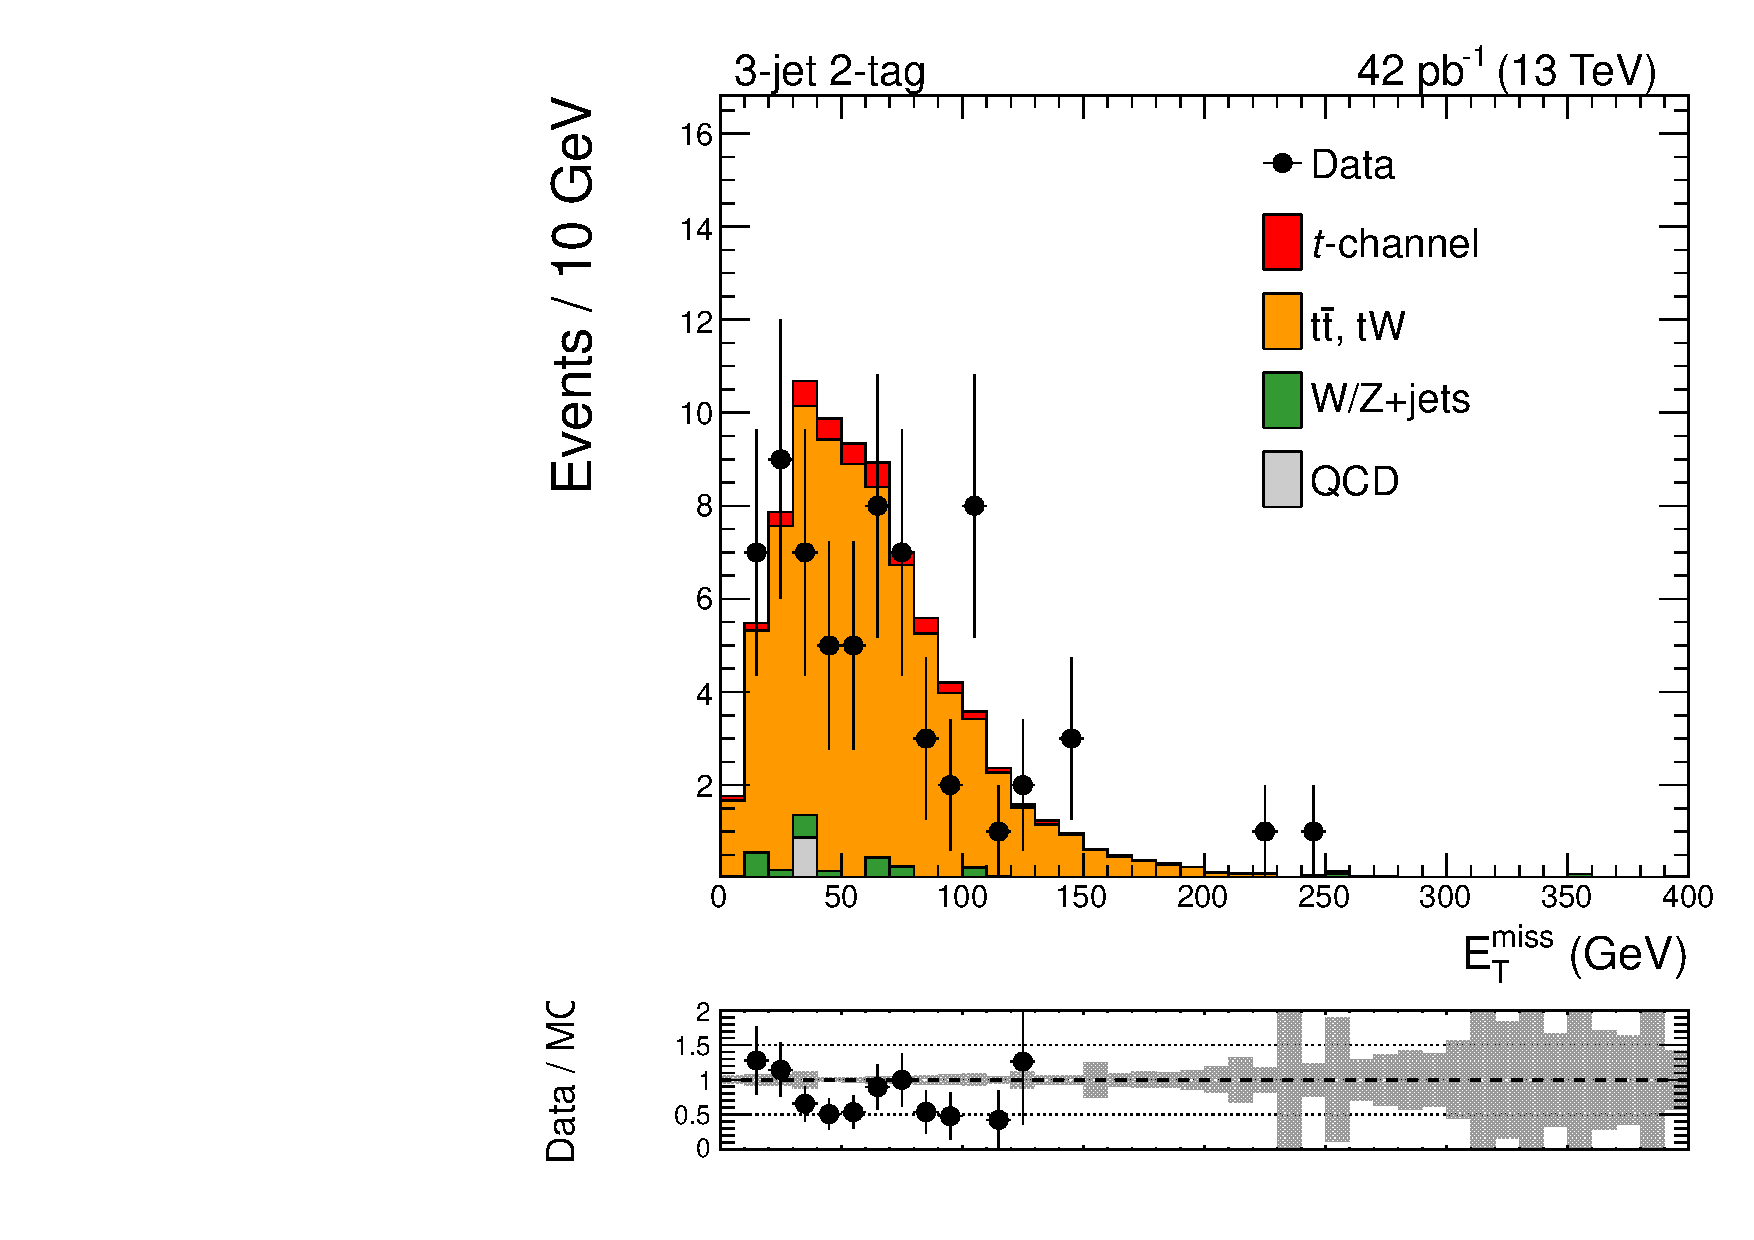
\includegraphics[width=6.5cm]{figures/3J2T/3j2t_MET.pdf}
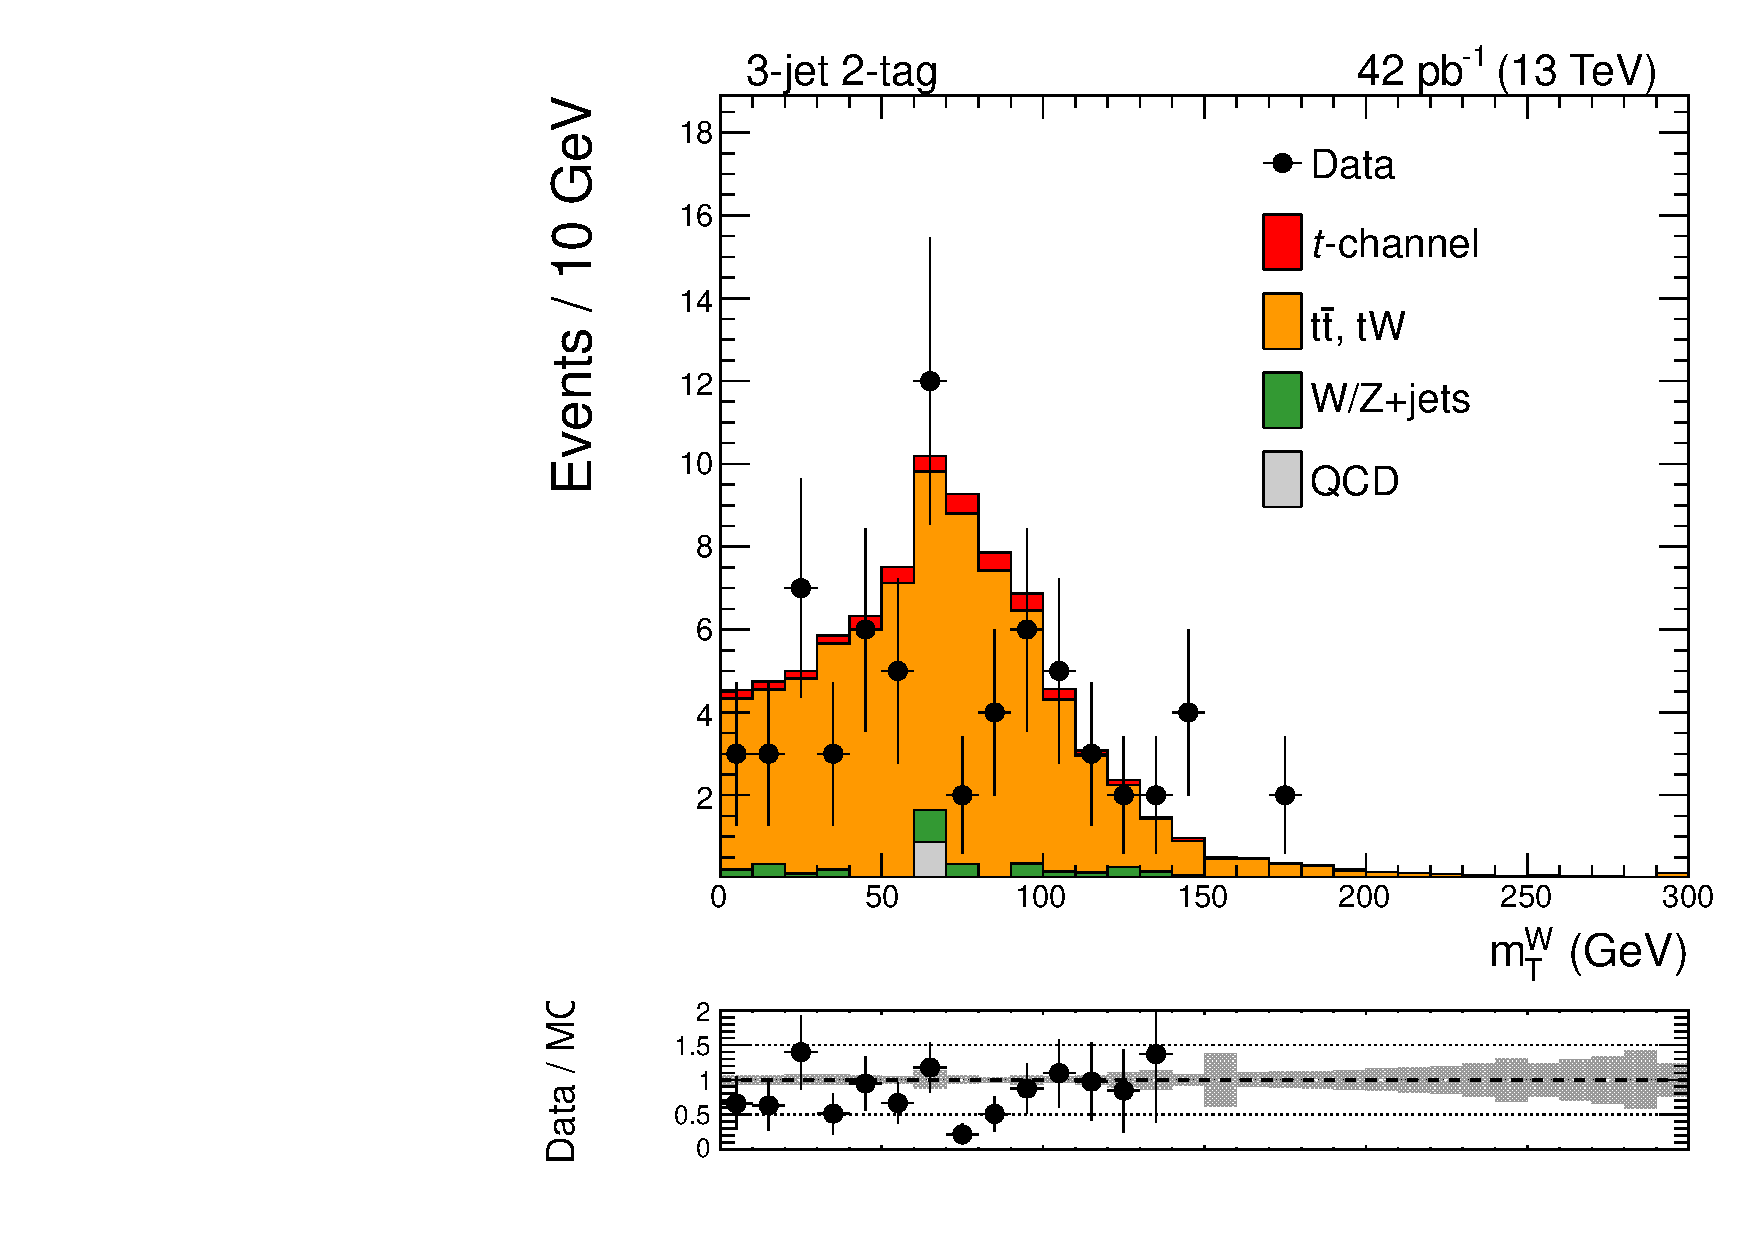
\includegraphics[width=6.5cm]{figures/3J2T/3j2t_mt.pdf}\hfill
\caption{\label{fig:Mu_MET_3J1T} Distributions of muon p$_{T}$ (upper left) and $\eta$ (upper right) and \met (lower left) and \mt (lower right) in the 3J2T region.}
\end{center}
\end{figure}




\begin{figure}[hbpt]
\begin{center}
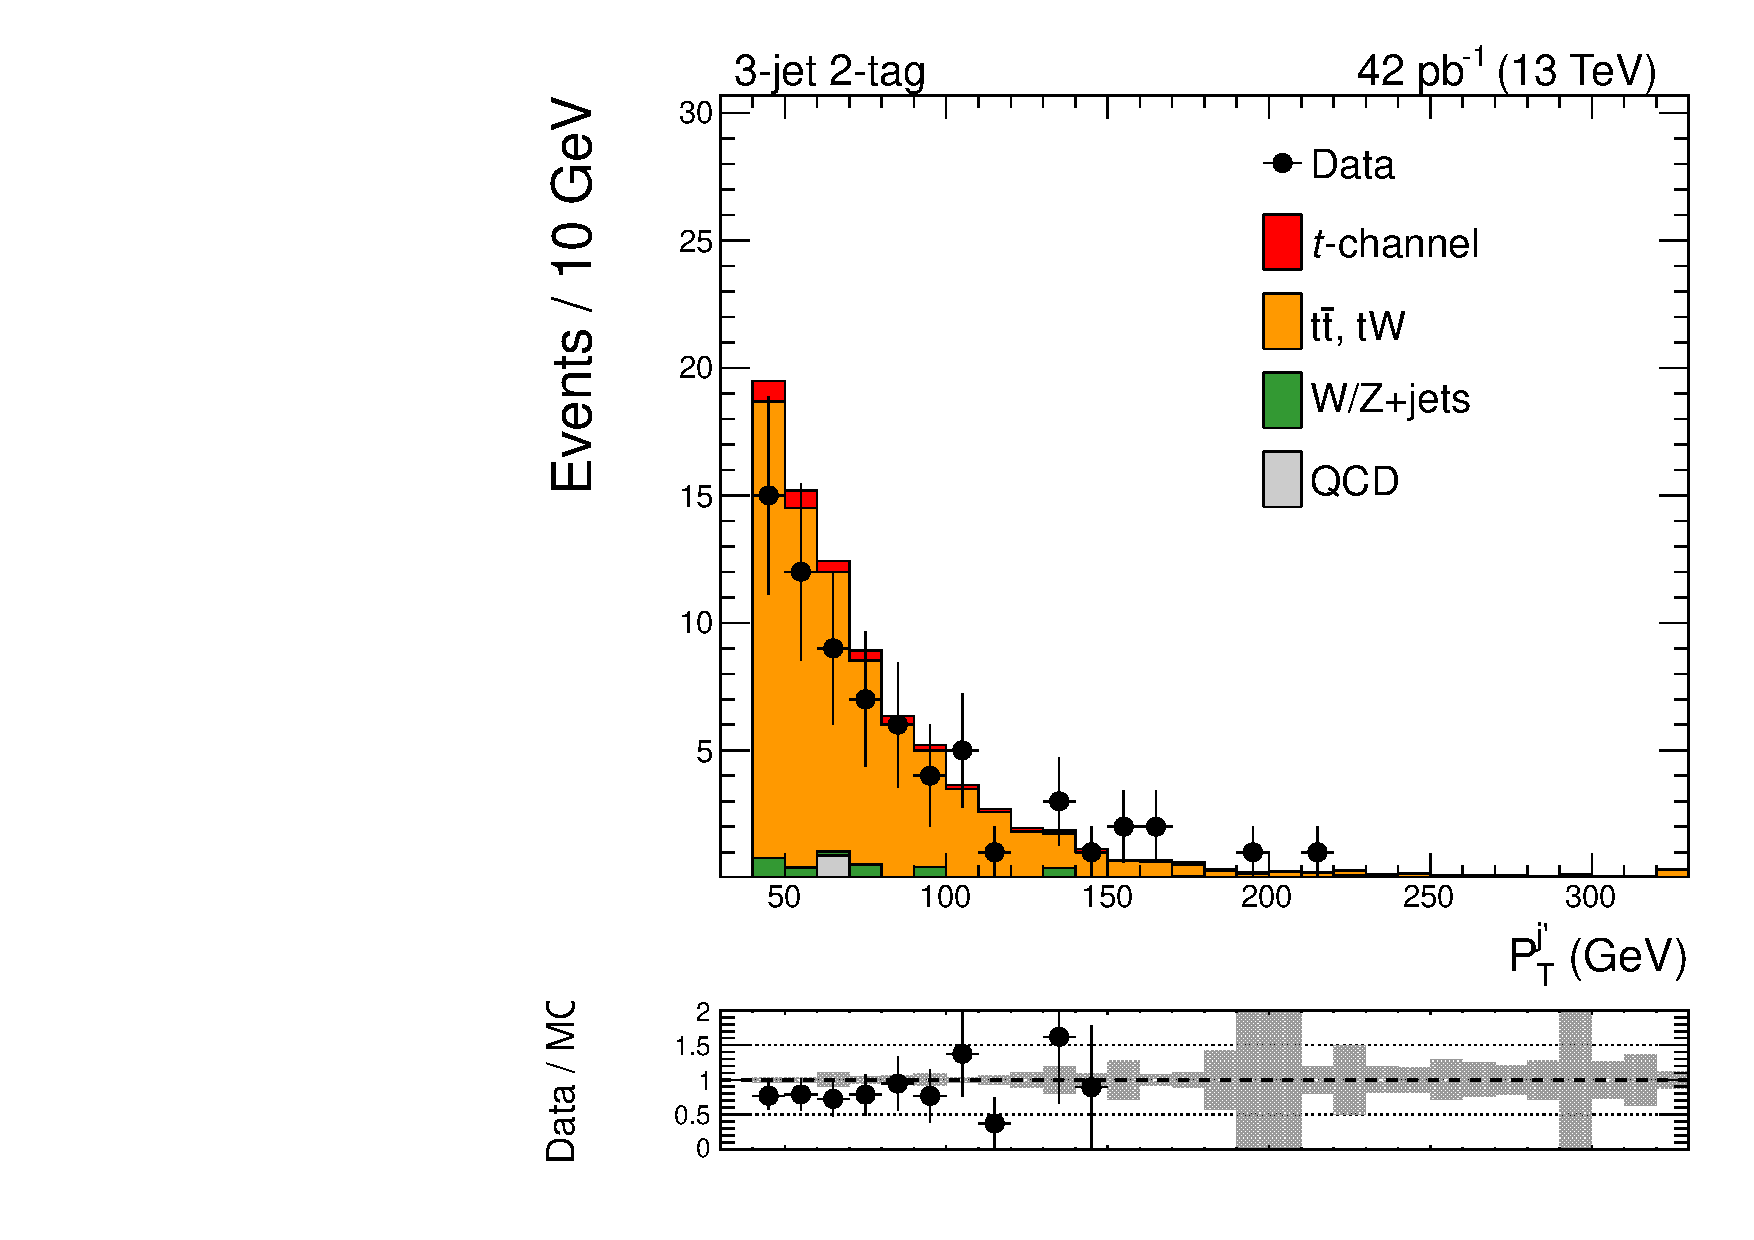
\includegraphics[width=6.5cm]{figures/3J2T/3j2t_ptjp.pdf}
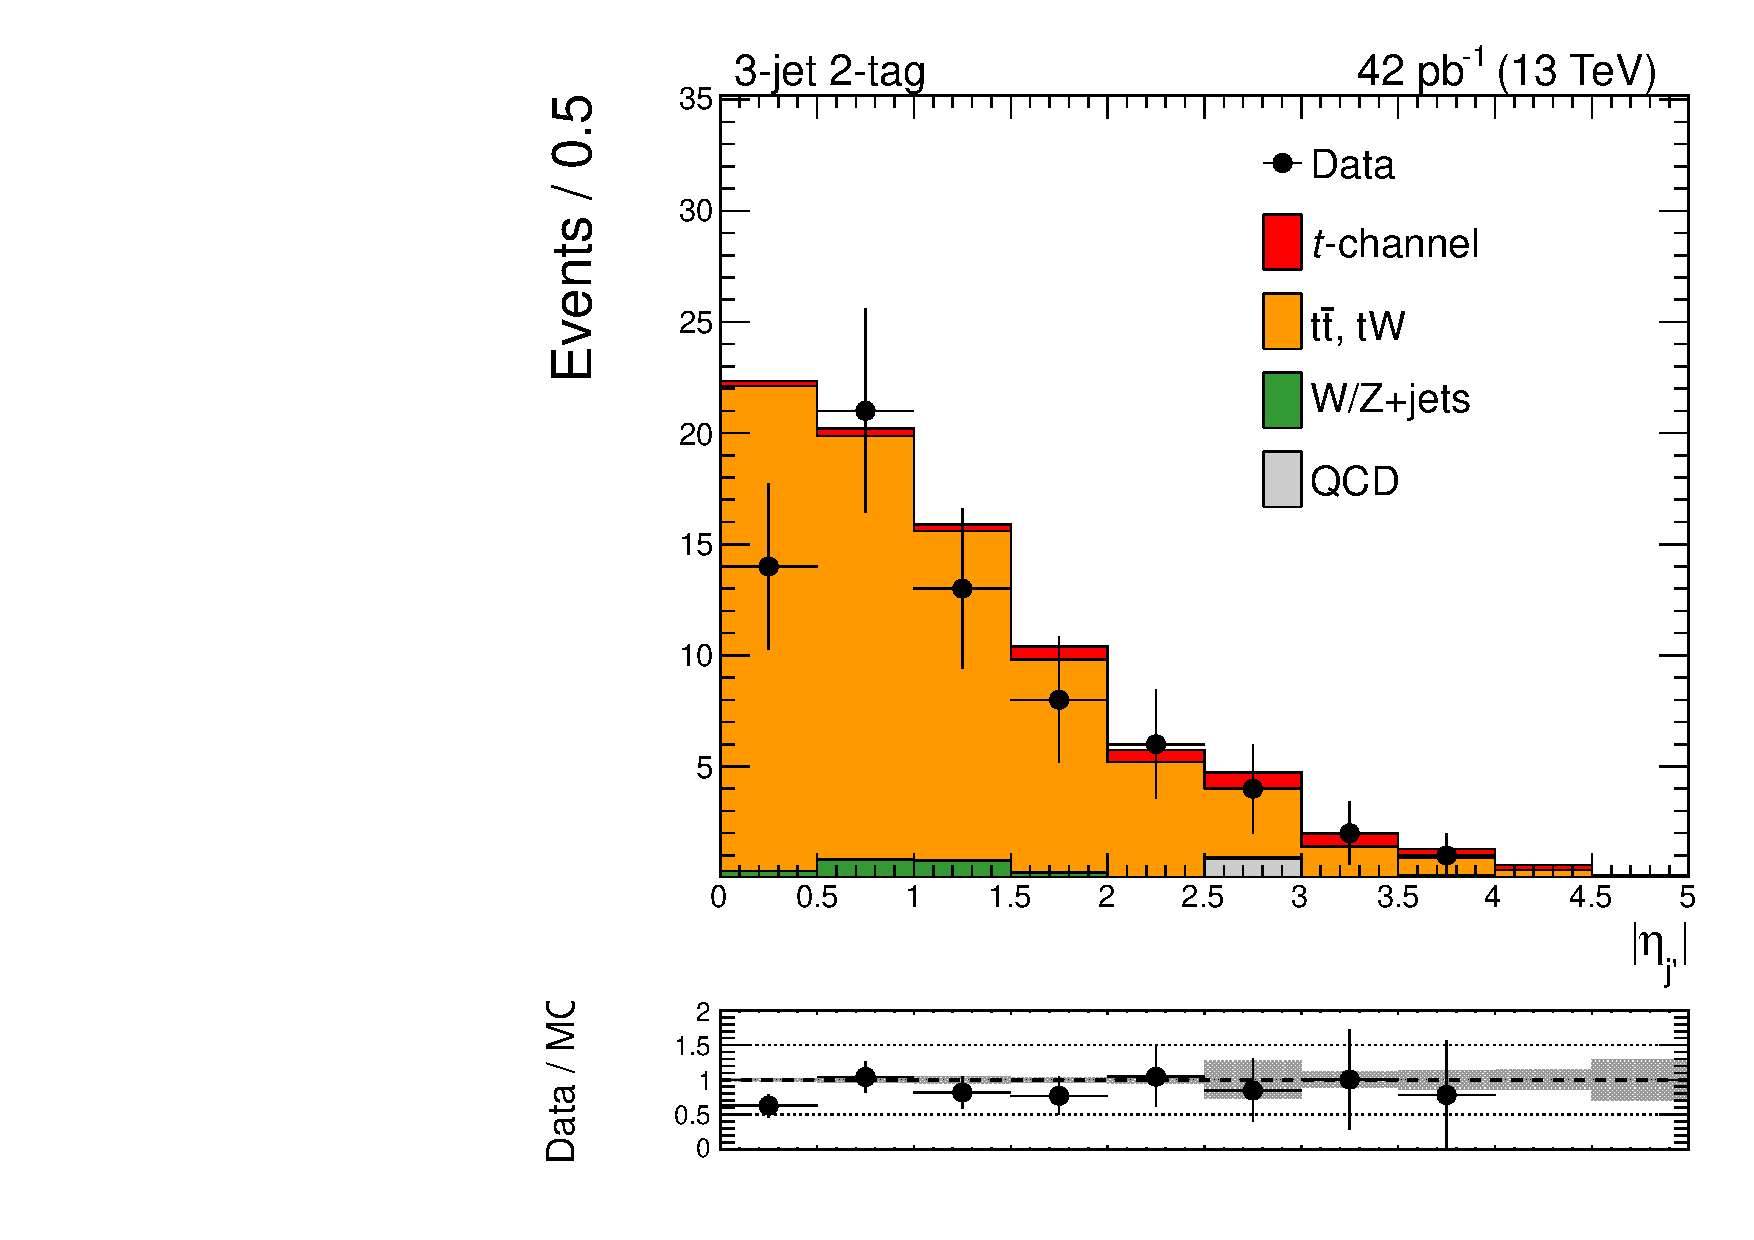
\includegraphics[width=6.5cm]{figures/3J2T/3j2t_etajp.pdf}
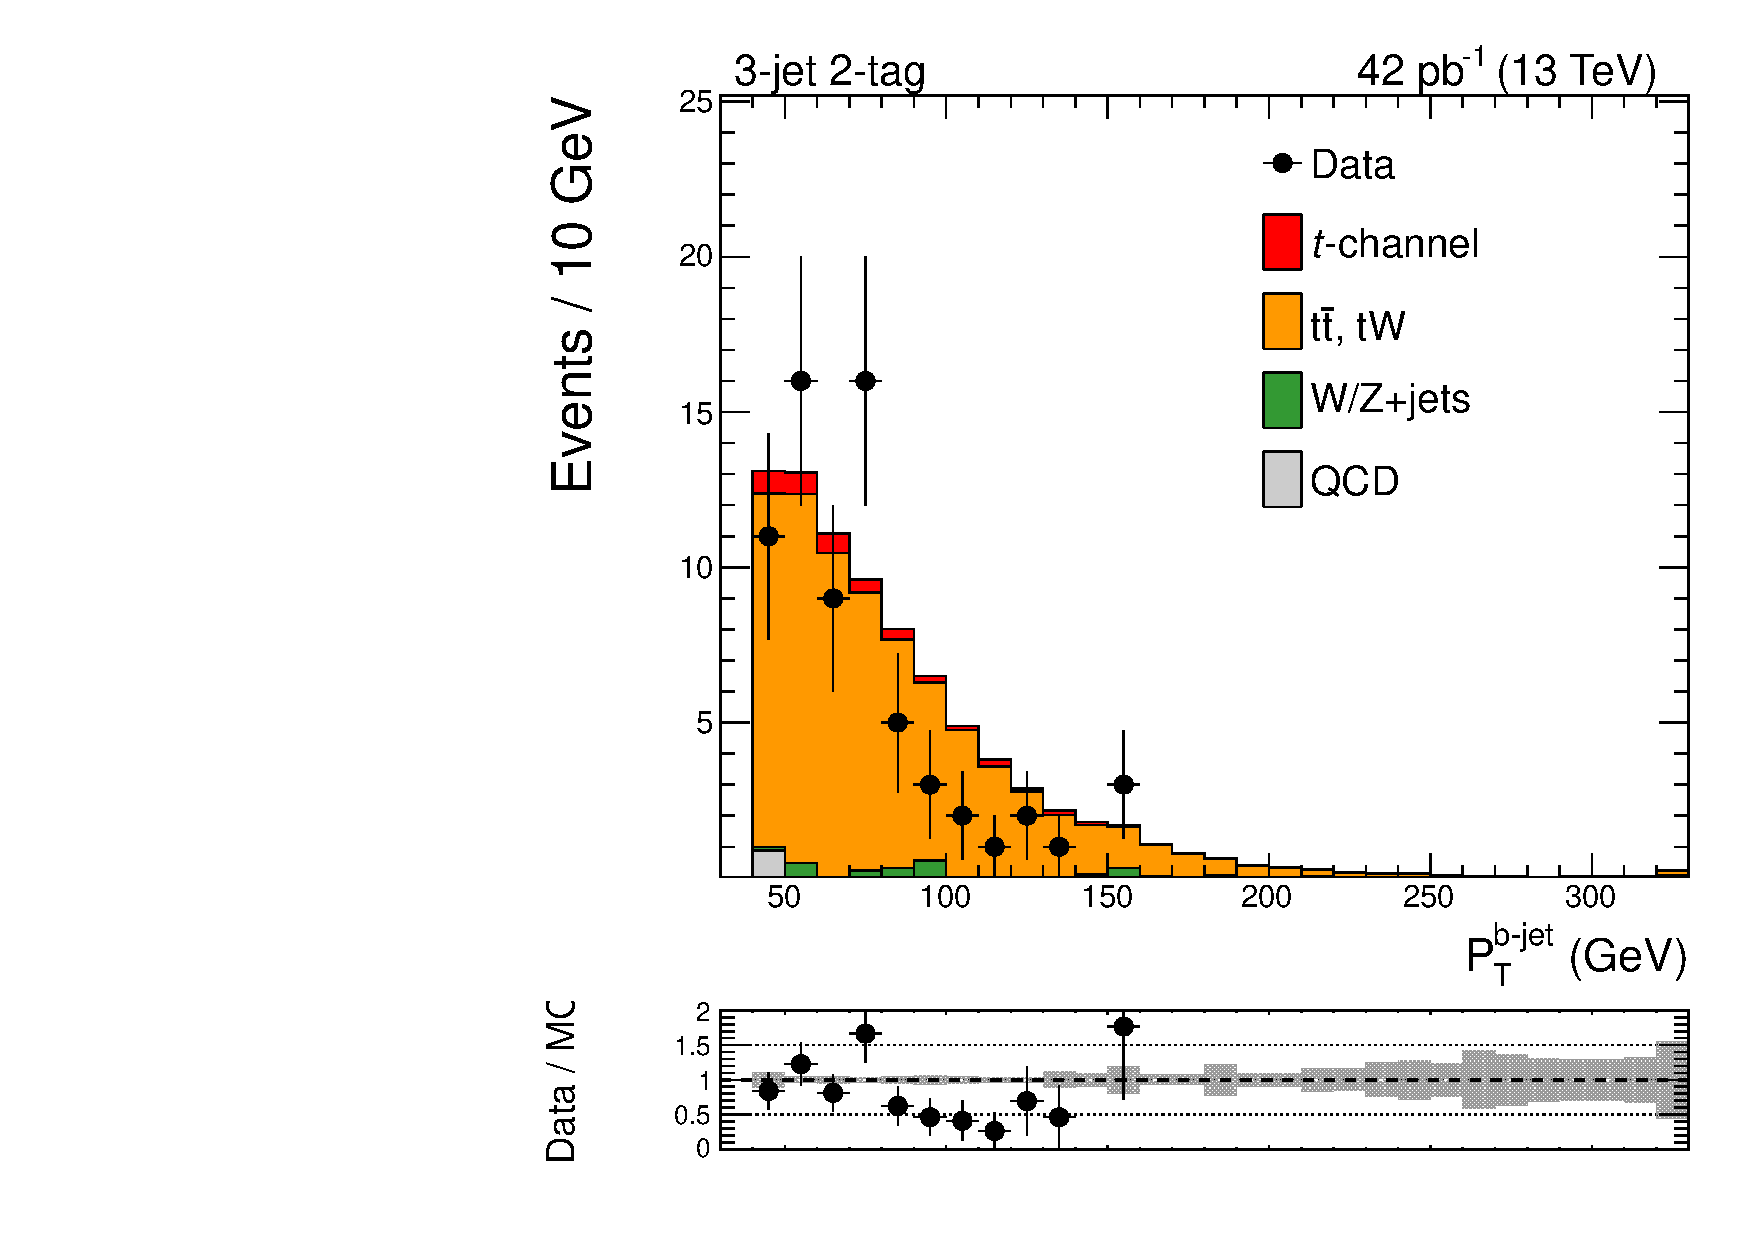
\includegraphics[width=6.5cm]{figures/3J2T/3j2t_bpt.pdf}
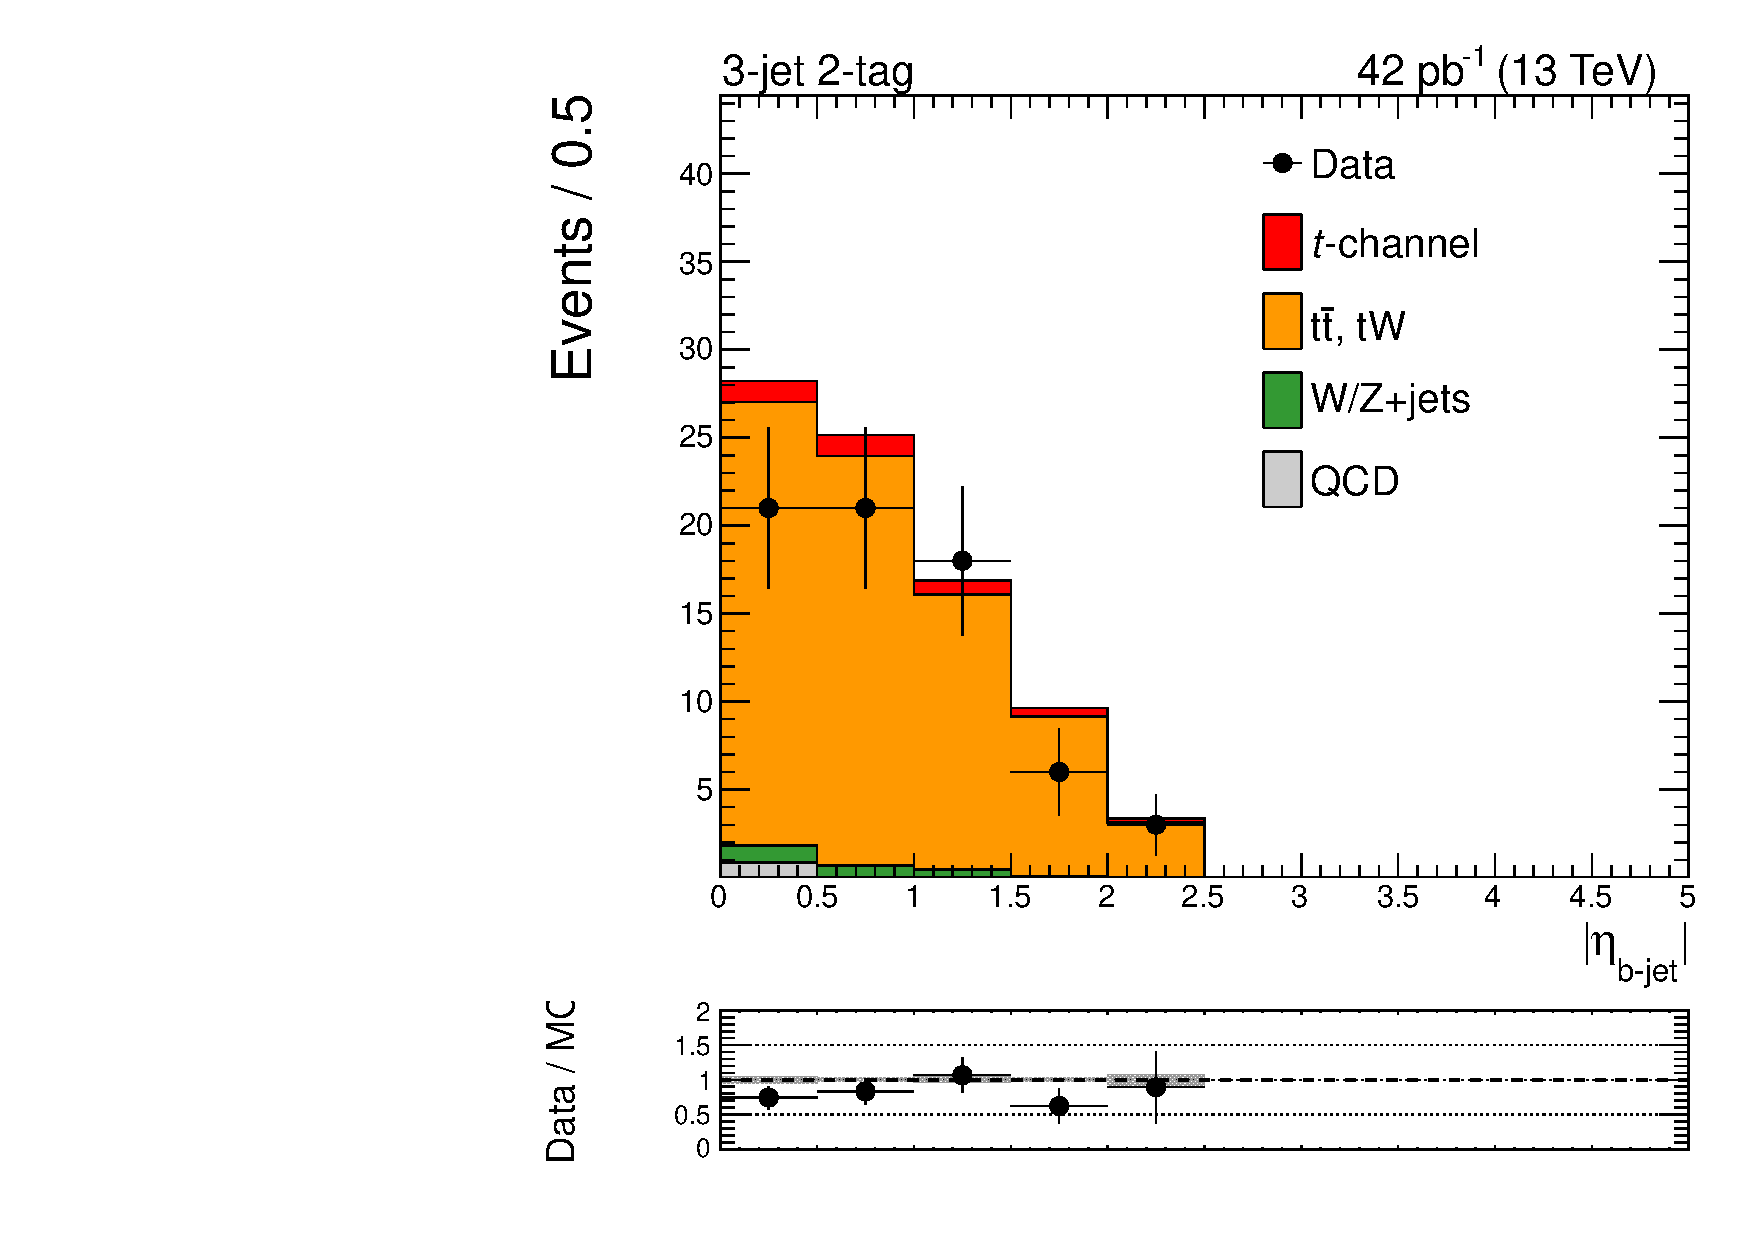
\includegraphics[width=6.5cm]{figures/3J2T/3j2t_beta.pdf}\hfill
\caption{\label{fig:Jets3J2T}p$_{T}$ (left) and $\eta$ (right) distributions of the non-tagged jet (upper row) and the b-tagged jet with the highest CSV-value in each event (lower row) in the 3J2T region.}
\end{center}
\end{figure}
